\section{Kältetechnischer Aufbau}
\label{sec:Kältetechnischer Aufbau}

In diesem Abschnitt werden die Teilsysteme des kältetechnischen Aufbaus vorgestellt. Der komplette kältetechnische Aufbau besteht aus der Kälteanlage mit dem Verdampfer-Prüfling und der Klimakammer, in der der Prüfling lokalisiert ist und unter verschiedenen Umgebungsgebenheiten getestet werden kann.

\subsubsection{Kälteaanlage}
\label{subsec:Kälteanlage}

\begin{figure}[htb]
\centering		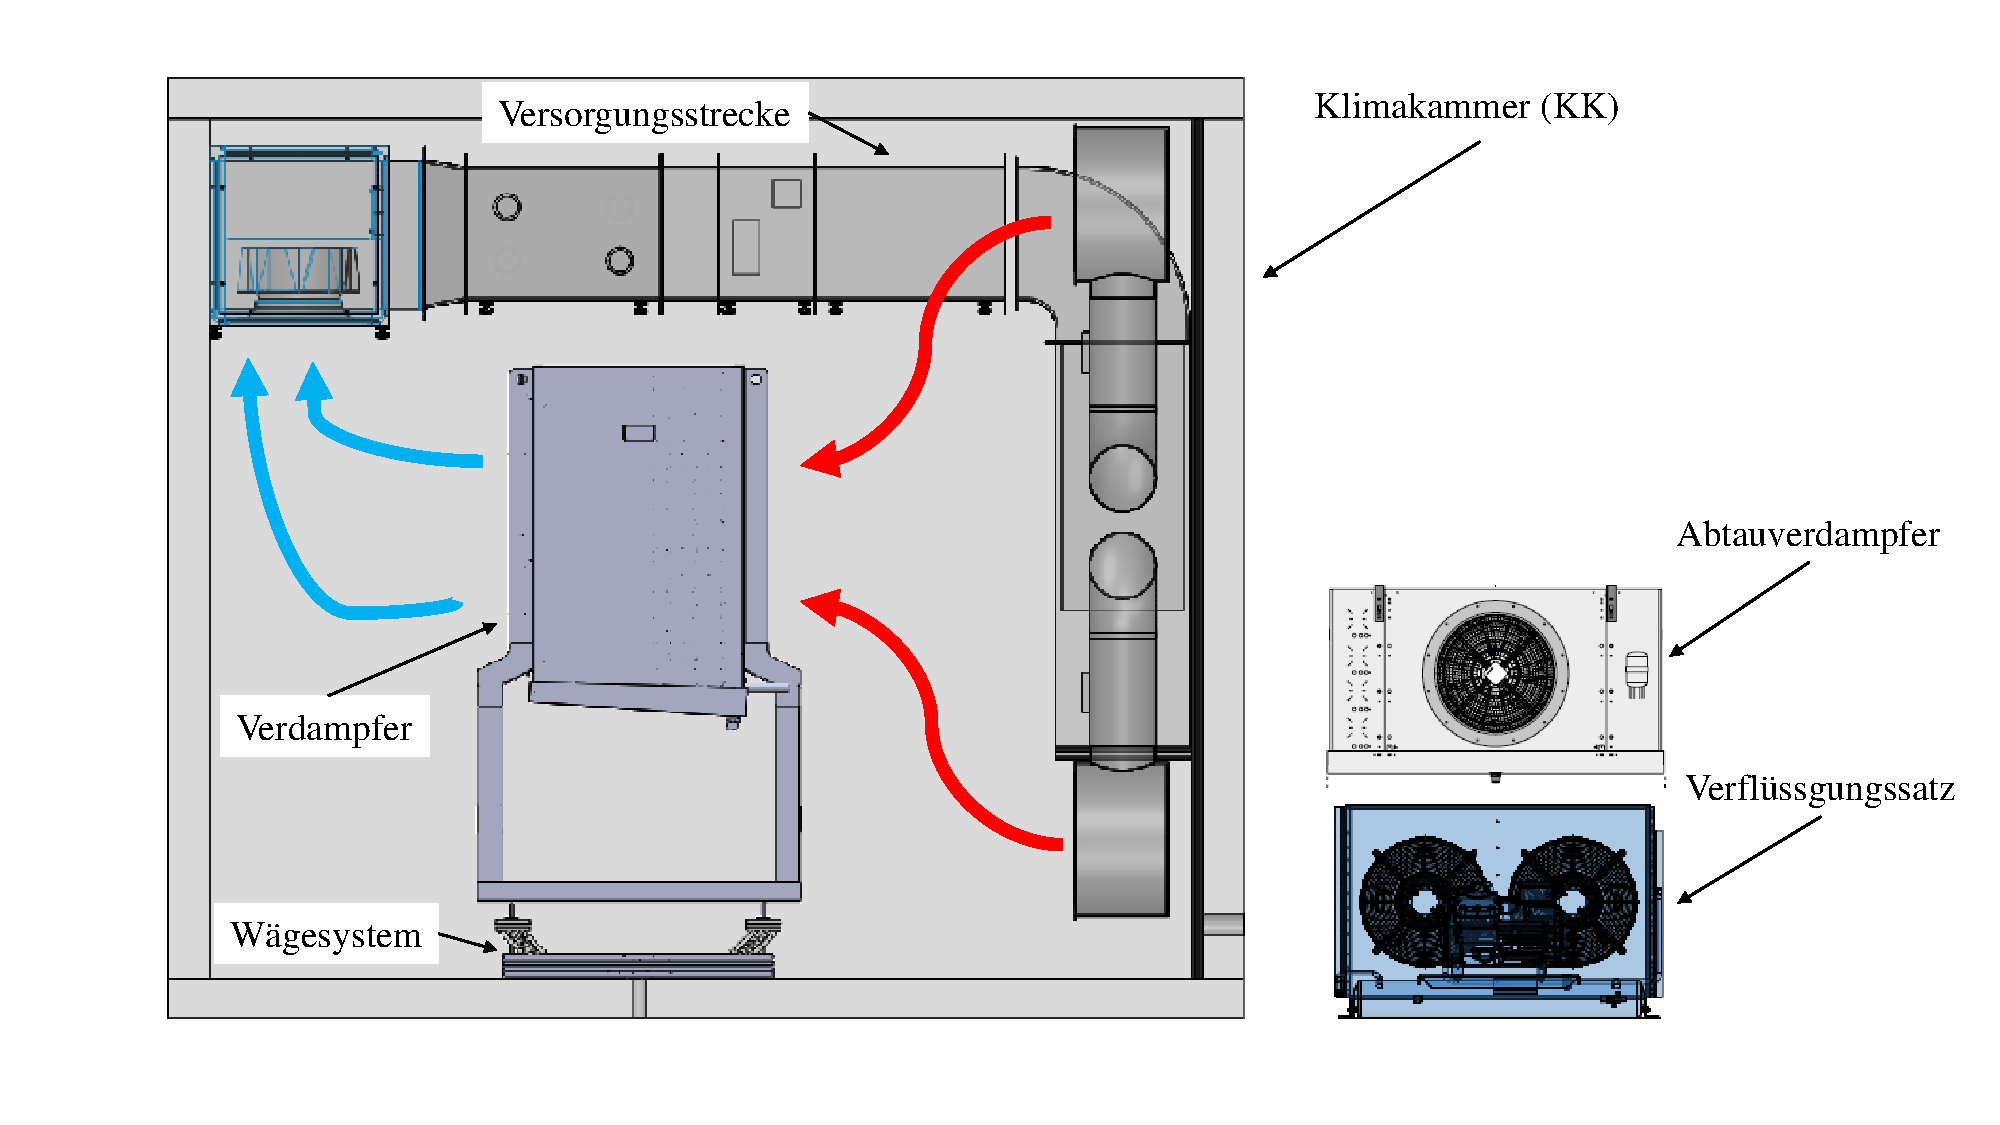
\includegraphics[page=1,width=0.90\textwidth]{Pictures/Versuchsaufbau/GesAufbau.pdf}
\caption{Gesamtaufbau mit Klimakammer, Luftkühler, Verflüssigungssatz und Wägesystem}
\label{fig:GesAufbau}
\end{figure}


Die Auslegungsdaten der Kälteanlage sind in Tabelle \ref{tab:Parameter KK} dargestellt. Abbildung \ref{fig:KA-Fliessbild}  zeigt das Fließschema der Kälteanlage. 


\begin{figure}[htb]
%\centering	
\includegraphics[ page=4, width=1.150\textwidth]{Pictures/RI.pdf}
\caption{RI-Fließbild der Kälteanlage}
\label{fig:KA-Fliessbild}
\end{figure}





Die Hauptkomponenten der Kälteanlage sind der Kompressor, der Verflüssiger, der Verdampfer und der Abtauverdampfer. Der Verflüssiger kondensiert im  Kühlbetrieb das überhitzte Kältemittel vollständig und der Abtauverdampfer verdampft das Kältemittel im Abtaubetrieb durch Prozessumkehrung, bevor es zurück in den Kompressor gesaugt wird. Der Verdampfer ist gleichzeitig der Prüfling, den es zu untersuchen gilt. Der Verdampfer ist durch die vorgesehenen Absperrventile austauschbar. Diese Vorrichtung ermöglicht unterschiedliche Bautypen von Luftkühlern zu testen. 

Danach gelangt das Kältemittel in den Ölabscheider, der einen großen Teil des Öls vom Kältemittel trennt und zurück zur Schmierung des Verdichters führt. Vor und nach dem Kompressor sind sowohl zur Energie-Bilanzierung als auch zwecks Anlagenschutz Temperatur- und Drucksensoren installiert. Dieser Vorgang ist im Abtau- und Kühlbetrieb identisch. 

Das Kältemittel, das aus dem internen Wärmeübertrager Richtung Kompressor gesaugt wird, passiert zunächst den Tropfenabscheider.  Der Tropfenabscheider stellt sicher, dass kein noch flüssiges Kältemittel in den Kompressor eindringt. Dies hätte verheerende Folgen für den Kompressor und wird genauer in Abschnitt \ref{sec:Informationstechnischer Aufbau} des Anlagenschutzes beschrieben. 

In der Klimakammer findet der Verdampfungsprozess statt. Neben dem Verdampfer ist hier das Expansionsventil installiert. Das Kältemittel wird im Kühlfall durch die Flüssigkeitsleitung eingespritzt und verlässt den Verdampfer über die Saugleitung. Im Abtaubetrieb durch Prozessumkehrung kann das Heißgas entweder durch die Venturidüse in den Verdampfer  oder durch die Saugleitung gelangen\footnote{In dem weiteren Verlauf der Arbeit wird von Heißgaseintritt über die Venturidüse von \textit{Oben} gesprochen, da der Wärmeübertrager aus vier Rohrlamellen-Wärmeübertragern besteht und die Einspritzung stets im obersten, rechten  Rohr geschieht. Von \textit{Unten} wird hingegen benutzt um die Variante mit Eingang des Heißgases über die Saugleitung zu beschreiben, da die Saugleitung stets das unterste Rohr ist.}. Die Abbildung \ref{fig:Magnetventil} sind die Varianten mit den Magnetventilstellungen abgebildet. 


\begin{figure}%[htb]
\centering		
\hspace{2cm}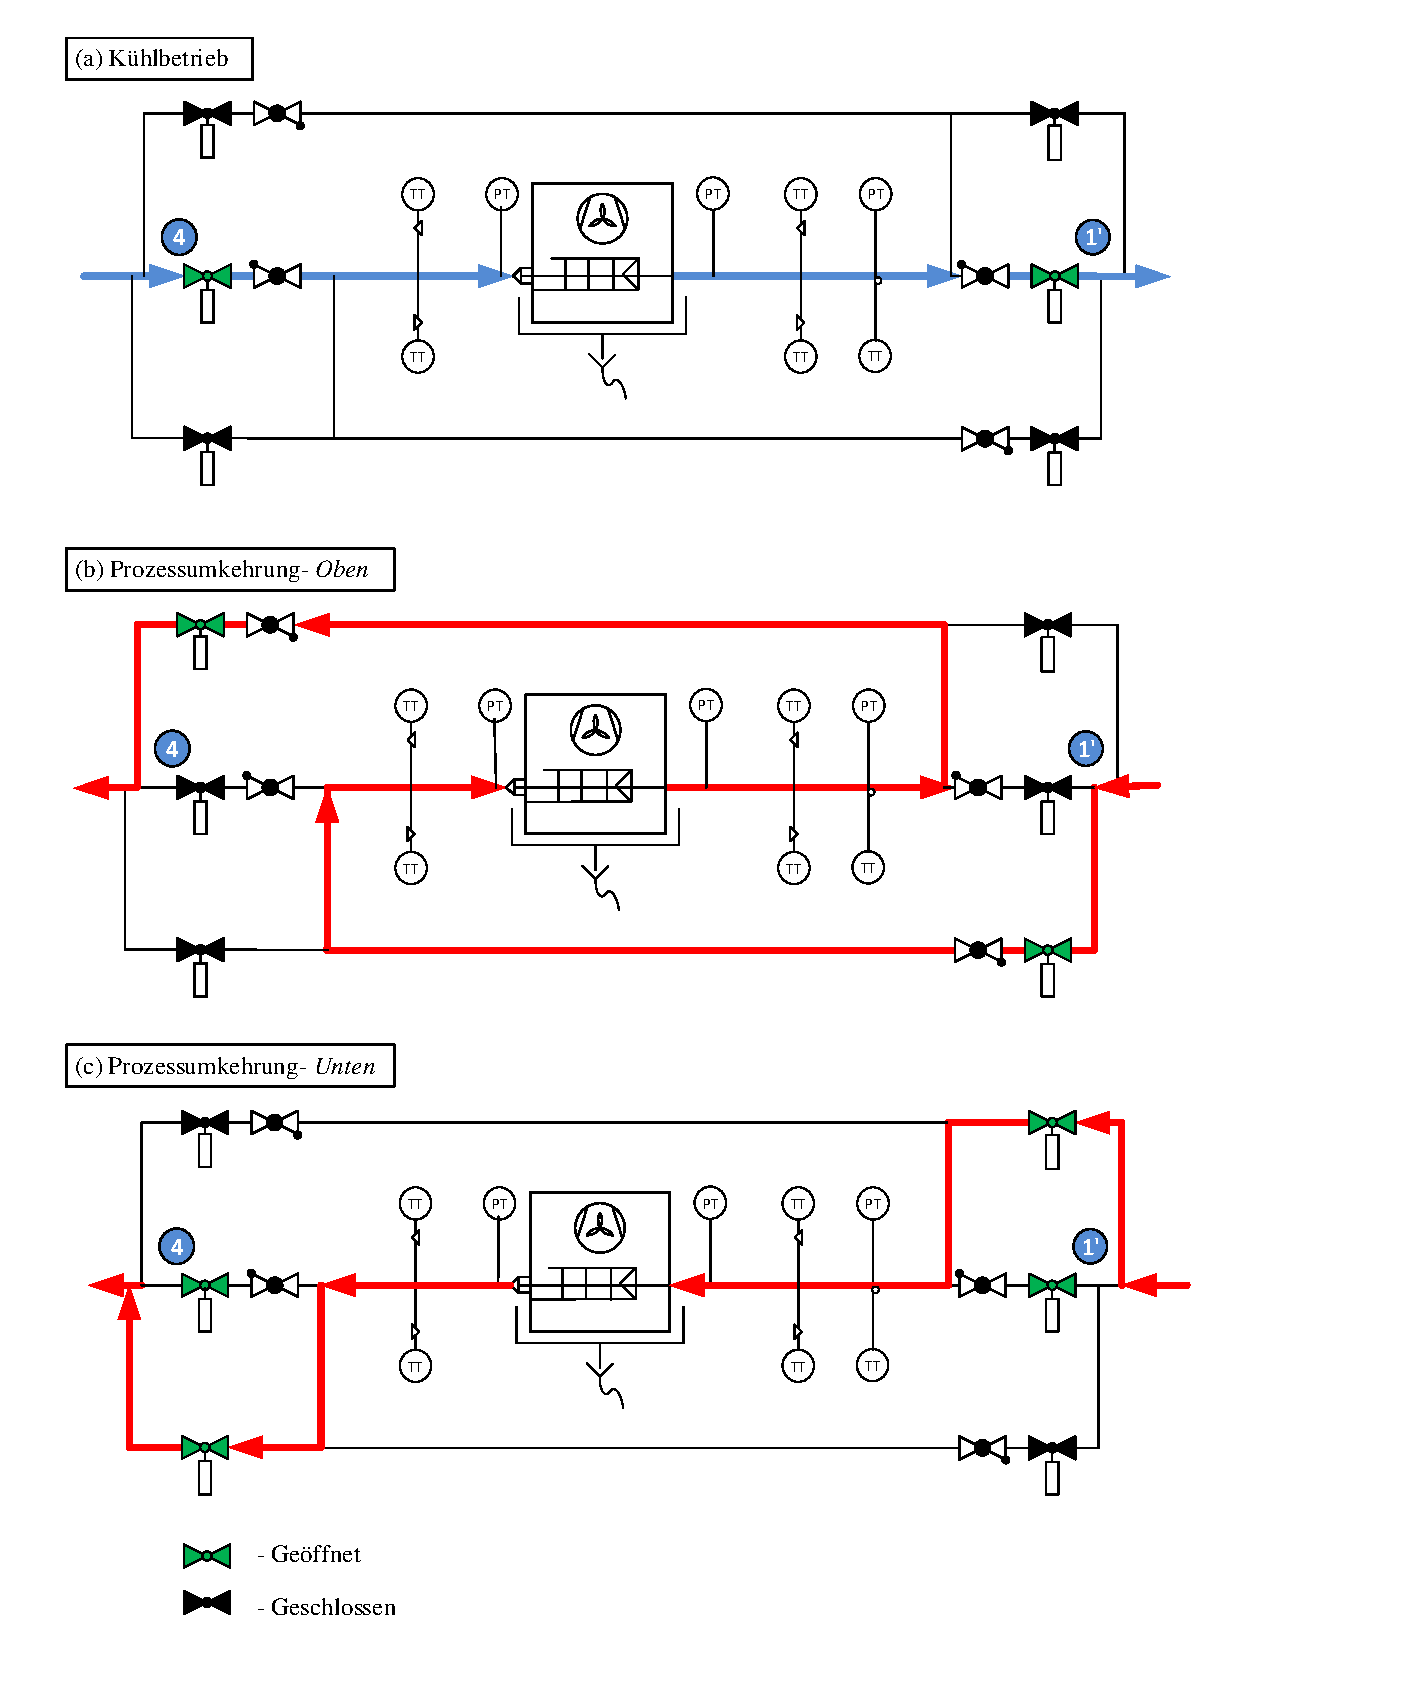
\includegraphics[width=1.15\textwidth]{Pictures/Schaltschema.pdf}
\caption{Mögliche Magnetventil-Schaltungen}
\label{fig:Magnetventil}
\end{figure}

\begin{table}[htb]
\centering
\caption{Auslegungsdaten des Verflüssigungssatzes laut Hersteller}\vspace{6pt}
\label{tab:Parameter KK}
\begin{tabular}{ll}
\hline 
\textbf{Systemparameter} & \textbf{Kälteanlage} \\ 
\hline 
\hline
Kältemittel & R134a\\
\hline
Verdampfungstemperatur & -8,0 °C\\
\hline
Verdampfungsdruck(abs) & 2,17 bar\\
\hline
Verflüssigungstemperatur & 40,2 °C\\
\hline
Verflüssigungsdruck(abs) & 10,23 bar\\
\hline
Sauggastemperatur & 2 °C\\
\hline
Verdichtungstemperatur &72,4 °C\\
\hline
Kälteleistung & 11,2 kW \\ 
\hline 
Verflüssigungsleistung & 15,3 kW\\
\hline
Leistungsaufnahme & 4,07 kW \\ 
\hline
Kälteleistungszahl & 2,74\\
\hline 
Kältemittel-Massenstrom & 0,077 kg/s \\ 
\hline 
max. Leistung der Lufterwämer & 2x 20 kW \\ 
\hline 
max. Kühlleistung & 10 kW \\ 
\hline 
Steuer- und Regelungstechnik & TWINCAT 3/ VB.NET \\ 
\hline 
\hline 
\end{tabular} 
\end{table}


\subsubsection{Kühlbetrieb, Zustandspunkte: $1 \rightarrow 2 \rightarrow 2'\rightarrow 3' \rightarrow 3''\rightarrow  3''' \rightarrow 3 \rightarrow 4 \rightarrow 1' $}

Im Kühlbetrieb strömt das flüssige unterkühle Kältemittel nach dem Verflüssiger erst in den Sammler. Danach überträgt es Wärme zwischen den Zustandspunkten $3''$ und $3'''$ an das aus dem Verdampfer kommende verdampfte Kältemittel. Am Zustandspunkt $3$ befindet sich der Massenstromsensor und ein Schauglas.  
Im \textbf{Kühlbetrieb} wird das Kältemittel durch das Expansionsventil entspannt und kurz vor dem Verdampfer durch eine Venturidüse ein weiteres Mal entspannt und eingespritzt.

\subsubsection*{Abtaubetrieb, Zustandspunkte: $1 \rightarrow 2 \rightarrow 1'\rightarrow 4 \rightarrow 3''\rightarrow  3''' \rightarrow 3 \rightarrow 3' \rightarrow 2' $}

Im Abtaubetrieb durch Prozessumkehrung fließt das Kältemittel, vom Verdampfer kommend, auch erst in den Sammler, um danach durch den internen Wärmeübertrager zum Massenstromsensor zu gelangen. Danach wird es über das Expansionsventil in den Abtau-Verdampfer eingespritzt. Rückschlagventile sind jeweils vor und nach einem Wärmeübertrager installiert. Rückschlagventile erlauben dem Kältemittel, nur in eine Richtung zu fließen. Dies ermöglicht, dass im Abtaubetrieb das Kältemittel durch den Abtauverdampfer geführt wird und dort verdampft. 







%\footnote{Mit Abtaubetrieb ist hier nur die Abtaumethode Prozessumkehrung gemeint. Bei der elektrischen Abtauung steht die Kältemaschine still und fährt erst nach dem Abtauprozess wieder an.} 



\subsubsection*{Messtechnik}
\label{subsubsec:Messtechnik}

Die Kälteanlage ist mit Temperatur-, Drucksensoren und einem Massenstromsensor ausgerüstet. Diese Sensoren dienen zur Bilanzierung der Wärmeübertrager und des Kompressors, spielen aber auch eine wichtige Rolle beim Anlagenschutz. In Tabellen \ref{tab:Messtechnik KA} sind die Sensordaten aufgeführt. 



\begin{table}[htb]
\centering
\caption{Sensordaten-Übersicht}\vspace{6pt}
\label{tab:Messtechnik KA}
\begin{tabular}{p{3cm}p{3cm}p{3cm}p{3.5cm}llll}
\hline 
 & \textbf{Drucksensor} & \textbf{Temperatursensor} & \textbf{Massenstromsensor} \\ 
\hline 
\hline 
Typ & PA 33 X & Pt100 & OPTIMASS 6400 C \\ 
\hline 
Hersteller & KELLER AG & CALOPLEX &  KROHNE Messtechnik GmbH \\ 
\hline 
Messbereich & 0$\dots$30 bar ~ \newline (0$\dots$10 bar) & -100$\dots$100 °C & 0$\dots$400 kg/h \\ 
\hline 
Messfehler & 0,01 $\%$ (10$\dots$40 °C)\newline 0,1 $\%$ (-10$\dots$80 °C) & 0,15 °C $\dots$ 0,35 °C  & 0,6 $\%$ \\ 
\hline 
Kommunikationsart & RS485 & 4$\dots$20 mA & RS485 \\ 
\hline 
Abfragefrequenz & 400 Hz & Busklemmen abhängig & Baudrate abhängig \\ 
\hline 
Hilfsenergie in V & 8$\dots$28 & - & 230  \\ 
\hline
Anzahl & 8  & 12 & 1 \\ 
\hline 
%Datenblatt(URL) & http://www.keller-druck.com/picts/pdf/german/33xg.pdf & • & https://www.instrumart.com/assets/Krohne-optimass6000-datasheet.pdf \\ 
\hline 
\end{tabular} 
\label{tab:Tabelle}
\end{table}
